%!TEX root = ../template.tex
%%%%%%%%%%%%%%%%%%%%%%%%%%%%%%%%%%%%%%%%%%%%%%%%%%%%%%%%%%%%%%%%%%%%
%% chapter5.tex
%% NOVA thesis document file
%%
%% Chapter with lots of dummy text
%%%%%%%%%%%%%%%%%%%%%%%%%%%%%%%%%%%%%%%%%%%%%%%%%%%%%%%%%%%%%%%%%%%%

\typeout{NT FILE chapter5.tex}%

\chapter{Simulation Framework}
\label{cha:simulations}

\epigraph{
	Whenever there is a problem, it usually lies between the chair and the monitor.
}

Simulations are a fundamental component of modern nuclear physics experiments, providing a virtual environment where experimental setups, detector responses, and physical processes can be modeled and tested prior to data acquisition. The simulation work for this thesis relies on three key software tools: Geant4, ROOT, and R3BRoot. Together, they form a comprehensive framework that enables the design, implementation, analysis, and validation of realistic nuclear experiments. The following subsections provide a brief overview of each tool and their respective roles in this work.

The simulation work in this thesis was conducted using the R3BRoot framework, the dedicated simulation and analysis environment developed for experiments within the \gls{R3B} collaboration. While R3BRoot was the only framework used directly, it is built upon two widely used and powerful tools in nuclear and high-energy physics: Geant4 and ROOT. A brief overview of these tools is presented here to provide context for the capabilities offered by R3BRoot.

\begin{figure}
	\centering
	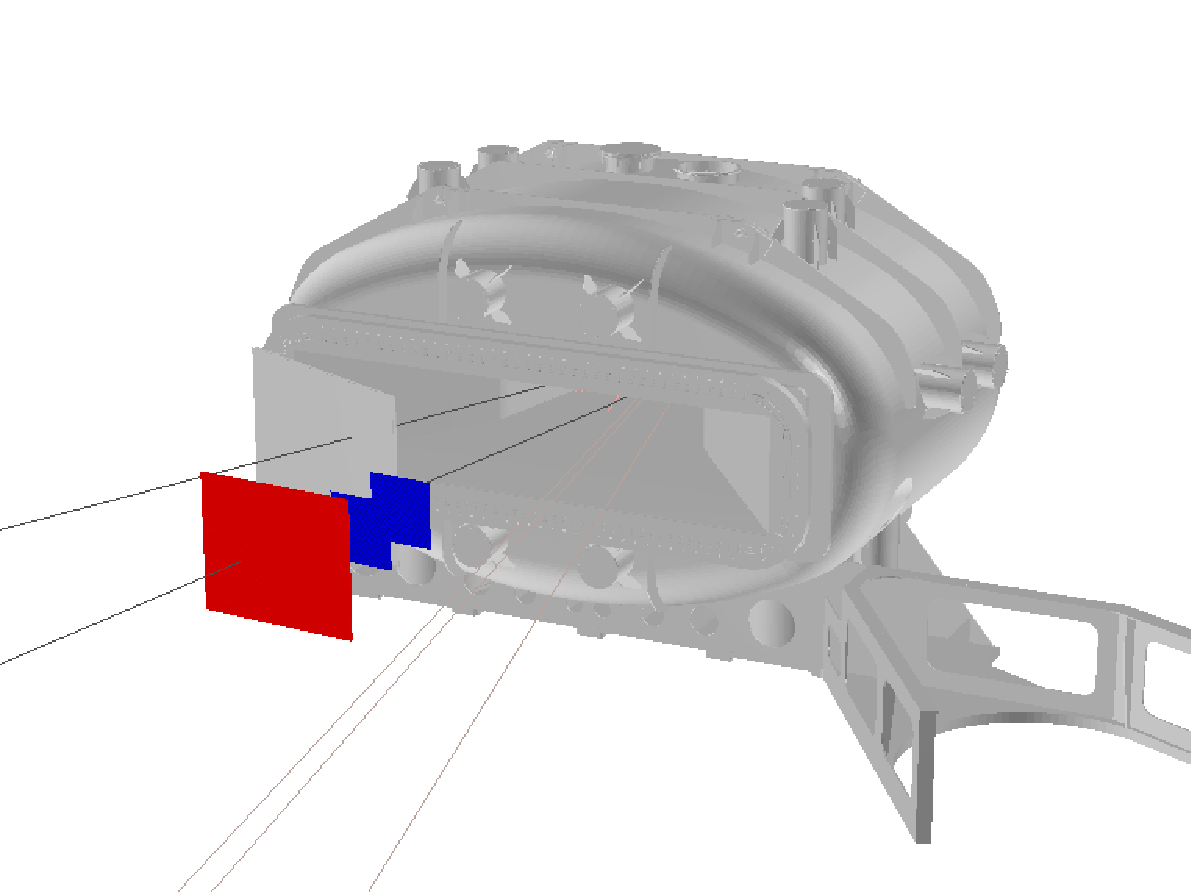
\includegraphics[width=0.6\linewidth]{/Simulations/SimEvEx}
	\caption{Example of an event in a simulation. In this case, there's a $^{14}$C passing through ToFD, a Deuteron passing through the RPC and 3 neutrons going to NeuLAND.}
	\label{fig:Simulation}
\end{figure}

\section{Geant4}

Geant4 \cite{agostinelli_geant4simulation_2003} is a C++ toolkit developed by CERN for simulating the passage of particles through matter. It provides detailed physics models and tracking capabilities that allow for realistic modeling of particle interactions, energy loss, multiple scattering, and nuclear processes. Within R3BRoot, Geant4 is responsible for handling the physical transport of particles through the simulated experimental setup, including interactions with detector materials, magnetic fields, and other components. This embedded use of Geant4 ensures that the simulations reflect the underlying physics of the experiment with high fidelity.


\section{ROOT}

ROOT \cite{brun_root_1997} is an object-oriented data analysis framework that provides tools for statistical analysis, histogramming, visualization, and data storage. R3BRoot integrates ROOT to manage event data, apply reconstruction algorithms, visualize results, and store output in ROOT-compatible formats. ROOT’s capabilities are essential for handling the large volumes of simulated data produced and for performing the subsequent analysis and validation steps.


\section{R3BRoot}

R3BRoot \cite{bertini_r3broot_2011} is the main framework used throughout this thesis for performing all simulation and analysis tasks. Developed specifically for experiments at the \gls{R3B} setup, R3BRoot builds on the FairRoot framework and incorporates both Geant4 and ROOT. It provides pre-configured detector geometries, digitization routines, reconstruction algorithms, and analysis tools tailored to the \gls{R3B} experimental environment.

Using R3BRoot, detailed simulations of the $^{25}$F(p,2p)$^{24}$O experiment were performed, including particle generation, tracking through the GLAD magnet, propagation through the tracking detectors and the \gls{RPC}, and emulation of detector responses. The framework also allowed the incorporation of realistic detector resolutions and systematics, enabling the generation of data that closely mirrors what will be observed experimentally. This simulated data formed the basis for developing and validating the Multidimensional Fitting functions presented in this thesis.

\section{Plots}

\section{Multidimensional Fitting}

In experiments like those conducted with the \gls{R3B} setup, the information directly recorded by detectors is often insufficient on its own to fully reconstruct the physical quantities of interest. Raw observables such as hit positions and times must be interpreted in the context of the particle’s full trajectory, charge, and energy. To bridge this gap, multidimensional fitting (MDF) methods are used. These tools allow us to model complex, nonlinear relationships between measurable detector signals and the underlying physical properties of particles.

Multidimensional fitting is particularly powerful in the context of quasi-free scattering reactions, such as the one studied in the $^{25}$F(p,2p)$^{24}$O experiment. Given the diversity and overlap of signals produced by different particles and trajectories in the \gls{R3B} setup, MDF enables a more accurate reconstruction of particle kinematics by using correlated detector data. It also allows us to compensate for the intrinsic limitations of individual detectors by combining information from multiple systems.

\subsection{Application to the RPC and FOOT Detectors}

In the simulation phase of this work, MDF techniques were employed to enhance the reconstruction of particle kinematics at the \gls{RPC} detector — the main focus of this thesis. To train the fitting models, a realistic dataset was generated by simulating the propagation of particles expected to be detected in the experiment, namely protons, alpha particles, deuterons, and $^3$He nuclei. These particles were tracked from their production near the target, through the downstream tracking detectors (FOOTs), the GLAD magnet, and finally to the \gls{RPC}.

Nine input variables were selected to capture the relevant kinematic and spatial information of the particles:
\begin{enumerate}
	\item The x, y, z positions at the first FOOT detector;
	\item The directional angles of the particles (Tx and Ty), calculated from the positions at the first and second FOOTs;
	\item The x, y, z positions at the \gls{RPC};
	\item The time of flight between the last FOOT and the \gls{RPC}.
\end{enumerate}


These features encapsulate the spatial evolution and timing of the particle along its flight path, providing the necessary information to infer more abstract physical quantities.

Four distinct MDF functions were trained using this dataset:

\begin{itemize}
	\item A function to estimate the momentum over charge (p/Q) of the particle;
	\item One function to estimate the momentum in x and another the momentum in y of the particle;
	\item A function to estimate the flight path (i.e., the actual distance traveled by the particle between the production point and the \gls{RPC}).
\end{itemize}


Each function was trained separately to isolate specific aspects of the particle’s motion and improve precision. These trained models can later be applied to experimental data to infer momentum and trajectory parameters with higher confidence than would be possible using analytic approximations alone.

This approach demonstrates the importance of data-driven tools like MDF in modern nuclear physics experiments, where complexity and high dimensionality make traditional reconstruction methods insufficient.

\subsection{Validation of the MDF Models}

Once the MDF models were trained, their performance was validated using a new set of Geant4 simulations that modeled a realistic experimental scenario. These simulations incorporated realistic beam-target reactions and included detector resolution effects, reproducing the uncertainties expected in the actual experiment.

For each simulated event, detector observables were extracted and fed into the trained MDF functions, which returned reconstructed values of the physical parameters. These were then compared against the known "true" values from the simulation. The difference between predicted and simulated values was analyzed through a series of performance plots.

The results demonstrated high predictive accuracy of the MDF functions. The residuals between predicted and true values were typically small, with uncertainties reaching down to the order of 10$^{-3}$ in normalized units. This level of precision confirms that the trained functions are robust and reliable, making them suitable for application to real experimental data in the analysis phase.

The successful validation of these MDF models underscores their value as a reconstruction tool in complex experimental setups like \gls{R3B}. They offer a data-driven approach to extracting meaningful physical insights from otherwise limited detector measurements, playing a central role in the broader simulation and analysis workflow of this thesis.


\section{Conclusions for the Experiment}